\documentclass[conference,10pt]{IEEEtran}
\usepackage{amsmath,amssymb}
\usepackage{booktabs}
\usepackage{tabularx}
\usepackage{multirow}
\usepackage{array}
\usepackage{graphicx}
\usepackage{tikz}
\usetikzlibrary{arrows.meta,positioning,fit,shapes.geometric}
\usepackage{xcolor}
\usepackage{microtype}
\usepackage{xspace}
\usepackage{url}
\usepackage[hidelinks]{hyperref}
\hypersetup{
  pdftitle={A Survey of KV-Cache Reuse and Hierarchical Memory Systems for Code Agents},
  pdfauthor={Project Research Team},
  pdfsubject={Independent technical survey of Code Agent workloads, KV-cache reuse, and hierarchical memory systems},
  pdfkeywords={Code Agent, KV-cache, prefix caching, context reuse, hierarchical memory, LLM serving}
}

\newcolumntype{Y}{>{\raggedright\arraybackslash}X}
\newcommand{\kvcache}{KV-cache\xspace}
\newcommand{\ttft}{TTFT\xspace}
\newcommand{\tpot}{TPOT\xspace}
\AtBeginEnvironment{thebibliography}{\setlength{\hfuzz}{1pt}}

\title{A Survey of KV-Cache Reuse and Hierarchical Memory Systems for Code Agents}

\author{\IEEEauthorblockN{Project Research Team}
\IEEEauthorblockA{Independent Technical Survey\\
August 2026}}

\begin{document}
\maketitle

\begin{abstract}
Code agents repeatedly invoke large language models while reading repositories, calling tools, editing files, and observing tests. Their prompts are long, multi-turn, and partially repetitive, making them promising workloads for cross-request key-value (KV) cache reuse. The opportunity is also easy to overstate: textual repetition does not imply reusable attention state, cache transfer can be slower than recomputation, and cross-tenant sharing can create timing and reconstruction risks. This survey synthesizes 76 primary papers and 18 official technical documents available through August 30, 2026. It develops a Code Agent-specific taxonomy spanning exact-prefix caching, prompt canonicalization, position-independent and partial reuse, hierarchical HBM/DRAM/NVMe or remote storage, prefill-decode disaggregation, compression and eviction, and architecture-aware representations for MQA, GQA, MLA, sparse, and hybrid models. It separates logical hits from token and profitable hits, derives correctness and benefit conditions, compares representative systems, and proposes a trace-driven evaluation protocol. The evidence supports exact-prefix reuse plus deterministic context construction as the first reproducible baseline. Non-prefix reuse, low-bit storage, and deep hierarchies are promising but require explicit quality, latency, compatibility, and isolation validation. No public evidence currently establishes the project's proposed 95\% Code Agent hit-rate, 90\% hit-path \ttft reduction, or 10\% cost-ratio targets; these remain hypotheses for measurement.
\end{abstract}

\begin{IEEEkeywords}
Code Agent, KV-cache, prefix caching, context reuse, hierarchical memory, LLM serving, time to first token, cache quantization
\end{IEEEkeywords}

\section{Introduction}

Repository-level software engineering has become a representative agentic workload. SWE-bench asks a system to resolve real GitHub issues in executable repositories and explicitly exposes the need for multi-file reasoning, environment interaction, and long contexts \cite{jimenez2023swebench}. SWE-agent and OpenHands operationalize the closed loop: the model reasons, calls repository or shell tools, observes results, modifies state, and invokes the model again \cite{yang2024sweagent,wang2024openhands}. Agentless provides an important control because it replaces an open-ended agent loop with staged localization, repair, and validation \cite{xia2024agentless}. The comparison shows that ``Code Agent'' denotes a system and workload, not merely a code-generating model.

Repeated calls in one task often retain system instructions, tool schemas, repository rules, earlier messages, and unchanged files while appending a command result, test failure, or patch. Recomputing the entire prompt prefill wastes compute. Exact-prefix caching, implemented in production engines and APIs, can skip computation for an identical token prefix \cite{kwon2023efficient,zheng2023sglang,d01vllmproject,d07nvidia}. However, repository content is frequently reordered, compacted, filtered, or locally edited. A byte-identical code span appearing after a different prefix or at a different position generally has different hidden and KV states. CacheBlend, EPIC, and recent position-independent methods therefore introduce correction or selective recomputation rather than concatenating arbitrary cached tensors \cite{yao2024cacheblend,hu2024epic,ma2026irminsul}.

The systems problem is equally important. A cache hit in host memory, SSD, or a remote pool is only useful when lookup, transfer, restoration, and scheduling overheads are lower than local recomputation. MemServe, Mooncake, LMCache, Strata, and HiCache illustrate the movement toward distributed or hierarchical KV storage \cite{hu2024memserve,qin2025mooncake,liu2025lmcache,xie2025strata,d03sglangproject}. Compression and eviction can expand effective capacity, but approximate state may change output quality, and compressed layouts may lack high-throughput kernels \cite{liu2024kivi,hooper2024kvquant,gao2025rethinking}.

This survey addresses five research questions:

\begin{enumerate}
    \item Which properties of Code Agent trajectories create safe reuse opportunities?
    \item Under what execution identity and dependency conditions is cached KV reusable?
    \item How do exact-prefix, non-prefix, hierarchical, and compressed methods differ?
    \item Which metrics distinguish logical hits from performance and cost benefits?
    \item Which research gaps must be closed before ambitious hit-rate and cost targets can be treated as evidence?
\end{enumerate}

The contribution is not another generic catalog of KV compression. Existing reviews cover broad cache-consumption and acceleration techniques \cite{shi2024keep,li2024survey}. Here, the organizing object is the Code Agent trajectory and the interaction between context construction, serving semantics, memory hierarchy, architecture, and security.

\section{Review Method and Evidence Scope}

\subsection{Corpus Construction}

The survey used a structured search over arXiv, peer-reviewed proceedings, official project documentation, and references cited by seed systems. The cutoff date is August 30, 2026. Inclusion required a direct connection to at least one of five categories: (i) Code Agent workloads or repository benchmarks, (ii) prefix or position-independent reuse, (iii) hierarchical or disaggregated KV movement, (iv) compression, eviction, or attention architecture, and (v) evaluation or cache security. The final evidence set contains 76 papers and 18 official documents. Surveys were used for navigation; core claims were checked against primary papers or current official documentation.

Each item was assigned a project role and priority. Public availability was separated from redistribution permission: only papers with an explicit Creative Commons license were placed in the offline corpus. Other papers remain in the bibliographic index with direct official links. This distinction affects packaging, not scientific relevance.

\subsection{Evidence Levels}

Table~\ref{tab:evidence} separates evidence types. A paper's reported speedup is evidence for its own implementation and workload, not for an unseen Code Agent trace. Official documentation is authoritative for current interfaces but can change. Internal project targets are hypotheses until evaluated under a specified model, tokenizer, serving engine, hardware, concurrency, and cost model.

\begin{table}[t]
\caption{Evidence levels and permitted interpretation.}
\label{tab:evidence}
\centering
\small
\begin{tabularx}{\columnwidth}{p{0.08\columnwidth}p{0.31\columnwidth}Y}
\toprule
Level & Source & Use and limitation \\
\midrule
A & Peer-reviewed paper or formal proceedings & Core algorithm and system evidence; results remain configuration-specific. \\
B & Public preprint with methods and experiments & Emerging evidence; reproduction and later revision may be needed. \\
D & Official project or provider documentation & Current behavior, interfaces, metrics, and operational semantics. \\
P & Project target or internal hypothesis & Defines what to test; never reported as an achieved result. \\
\bottomrule
\end{tabularx}
\end{table}

\subsection{Threats to Literature Validity}

Three biases matter. First, recent systems often use different models, GPUs, block sizes, datasets, and latency definitions. Second, many compression papers emphasize memory ratios without production kernels or end-to-end request latency. Third, public Code Agent benchmarks measure task success, not token-level prompt overlap, cache location, or transfer time. The survey therefore emphasizes mechanisms and testable conditions over headline speedups.

\section{Code Agent Workloads}

\subsection{Working Definition}

A Code Agent is an LLM-centered software engineering system that can observe a repository and execution environment, select and invoke tools, modify project state, verify results, and iteratively decide the next action. The system usually contains an agent controller, context builder, model endpoint, tool interface, execution sandbox, and observation store. Claude Code's official description similarly centers repository reading, file editing, command execution, and development-tool integration \cite{d11anthropic}.

The model call at step $t$ can be abstracted as

\begin{equation}
P_t = S \Vert T \Vert R \Vert F_t \Vert H_t \Vert Q_t,
\label{eq:prompt}
\end{equation}

where $S$ is the system instruction, $T$ tool schemas, $R$ repository rules, $F_t$ selected files or code, $H_t$ dialogue and tool history, and $Q_t$ the current objective. After a tool call, $H_{t+1}$ typically appends an observation, while $F_t$ may change locally. Equation~\ref{eq:prompt} is a workload abstraction, not a claim that every framework uses this exact ordering.

\begin{figure}[t]
\centering
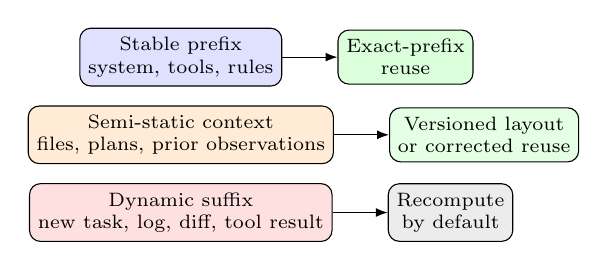
\begin{tikzpicture}[
  node distance=2.4mm,
  box/.style={draw,rounded corners,minimum height=5.5mm,align=center,font=\scriptsize,inner xsep=3pt},
  arr/.style={-{Latex[length=1.5mm]},thin}
]
\node[box,fill=blue!12] (stable) {Stable prefix\\system, tools, rules};
\node[box,fill=orange!16,below=of stable] (semi) {Semi-static context\\files, plans, prior observations};
\node[box,fill=red!12,below=of semi] (dynamic) {Dynamic suffix\\new task, log, diff, tool result};
\node[box,fill=green!14,right=7mm of stable] (exact) {Exact-prefix\\reuse};
\node[box,fill=green!10,right=7mm of semi] (versioned) {Versioned layout\\or corrected reuse};
\node[box,fill=gray!15,right=7mm of dynamic] (recompute) {Recompute\\by default};
\draw[arr] (stable) -- (exact);
\draw[arr] (semi) -- (versioned);
\draw[arr] (dynamic) -- (recompute);
\end{tikzpicture}
\caption{Prompt stability classes imply different cache semantics.}
\label{fig:stability}
\end{figure}

\subsection{Workload Diversity}

The SWE family now covers static, live, multilingual, multimodal, training, exploration, and long-horizon variants \cite{zhang2025swebench,zan2025multiswebench,pan2024training,yang2024swebench,zhang2026sweexplore,le2025sweevo}. RepoBench, RepoCoder, RepoFuse, and GraphCoder instead emphasize repository-level retrieval and completion \cite{liu2023repobench,zhang2023repocoder,liang2024repofuse,liu2024graphcoder}. ContextBench isolates the context-retrieval behavior of coding agents, while LongCLI-Bench studies long-horizon command-line programming \cite{li2026contextbench,feng2026longclibench}. These tasks create different repetition patterns and cannot be combined into one unqualified ``Code Agent hit rate.''

\begin{table*}[t]
\caption{Representative Code Agent workload families and cache-research value.}
\label{tab:workloads}
\centering
\small
\begin{tabularx}{\textwidth}{p{0.15\textwidth}p{0.21\textwidth}p{0.25\textwidth}Y}
\toprule
Family & Representative sources & Dominant interaction & Cache-research value \\
\midrule
Issue resolution & SWE-bench, SWE-bench Live, Multi-SWE-bench & Inspect repository, edit multiple files, run tests & Real execution loop; repository/version and test-output changes. \\
Agent platforms & SWE-agent, OpenHands & Model-directed shell, search, edit, and observation cycle & Exposes adjacent-call reuse and tool-schema stability. \\
Staged repair & Agentless & Localization, patch generation, validation & Control for separating open-ended agent overhead from task content. \\
Repository retrieval/completion & RepoBench, RepoCoder, RepoFuse, GraphCoder & Retrieve cross-file context and generate code & Tests deterministic file ordering and non-prefix code repetition. \\
Trajectory training & SWE-Gym, SWE-smith, long-context RL & Generate or learn from multi-step trajectories & Potential source of public traces and controlled replay workloads. \\
Long-horizon diagnostics & ContextBench, SWE-Explore, SWE-EVO, LongCLI-Bench & Explore, maintain state, and evolve code across many steps & Measures context churn, compaction, shifted reuse, and tail growth. \\
\bottomrule
\end{tabularx}
\end{table*}

\subsection{What Must Be Measured in a Trace}

The following quantities must remain distinct:

\begin{itemize}
    \item byte repetition and token repetition;
    \item longest common token prefix;
    \item repeated segments outside the prefix;
    \item reusable tokens under exact execution identity;
    \item tokens whose reuse is profitable from their current tier;
    \item task success, which can change under approximate reuse.
\end{itemize}

Recent agent studies strengthen the motivation but do not replace a target trace. Prompt caching has been evaluated for long-horizon agentic tasks, and trajectory reduction has been proposed to reduce agent cost \cite{lumer2026dont,xiao2025reducing}. Training work also confirms that software-engineering trajectories are long, multi-turn, and expensive to roll out \cite{golubev2025training,yang2025swesmith}. A project-specific trace must still capture the rendered prompt, tokens, segment boundaries, repository revision, model identity, cache events, and latency breakdown.

\section{KV-Cache Semantics and Correctness}

\subsection{Memory Model}

For a standard decoder Transformer, a first-order KV footprint is

\begin{equation}
M_{KV} \approx 2 L S H_{KV} d_h b,
\label{eq:kvsize}
\end{equation}

where $L$ is the number of layers, $S$ sequence length, $H_{KV}$ stored KV heads, $d_h$ head dimension, and $b$ bytes per element. The factor two accounts for keys and values. Batch size multiplies the result. MQA and GQA reduce $H_{KV}$; MLA stores a latent representation plus position-dependent components; sparse and hybrid models may store additional indexes or recurrent state \cite{shazeer2019fast,ainslie2023training,deepseekai2024deepseekv}.

PagedAttention reduces fragmentation and enables non-contiguous physical allocation \cite{kwon2023efficient}. vAttention instead preserves a contiguous virtual layout while allocating physical pages on demand \cite{prabhu2024vattention}. These are memory-management mechanisms; neither alone guarantees cross-request semantic reuse.

\subsection{Exact-Prefix Reuse Domain}

Let requests $a$ and $b$ share a token prefix $x_{1:k}$. Exact reuse is valid only if the execution identity is compatible. A practical cache key must cover at least

\begin{equation}
K = h(M,V,T,A,P,Q,D,x_{1:k},K_{parent},\Omega),
\label{eq:key}
\end{equation}

where $M$ is model family and weights, $V$ model revision, $T$ tokenizer, $A$ adapter or LoRA state, $P$ positional configuration, $Q$ attention and quantization layout, $D$ numerical dtype, $K_{parent}$ the prefix dependency, and $\Omega$ the tenant or security domain. Additional execution options may be necessary for a specific engine.

Block-hash chains in vLLM and radix-tree indexing in SGLang encode the dependence on earlier blocks \cite{d02vllmproject,zheng2023sglang}. Prompt Cache adds explicit reusable modules, while ChunkAttention combines a prefix-aware cache with a specialized attention kernel \cite{gim2023prompt,ye2024chunkattention}. Exact-prefix reuse should produce the same model state as recomputation, subject to the engine's numerical determinism and kernel behavior.

\subsection{Why Identical Text May Have Different KV}

For a causal Transformer, the hidden state at token $i$ depends on the preceding context. Moving a code block, changing a token before it, altering positions, or changing an adapter can change all downstream states. CacheBlend recovers non-prefix chunks by selectively recomputing influential tokens \cite{yao2024cacheblend}. EPIC uses position-independent compilation plus boundary repair \cite{hu2024epic}. MPIC extends position-independent ideas to multimodal contexts \cite{zhao2025mpic}. MEPIC, KV Packet, Irminsul, SparseX, and KVBoost represent a rapidly evolving family with different correction assumptions and architecture constraints \cite{wang2025mepic,chen2026packet,ma2026irminsul,zhang2026sparsex,unnikrishnan2026kvboost}. Their results do not justify generic tensor concatenation.

\begin{figure*}[t]
\centering
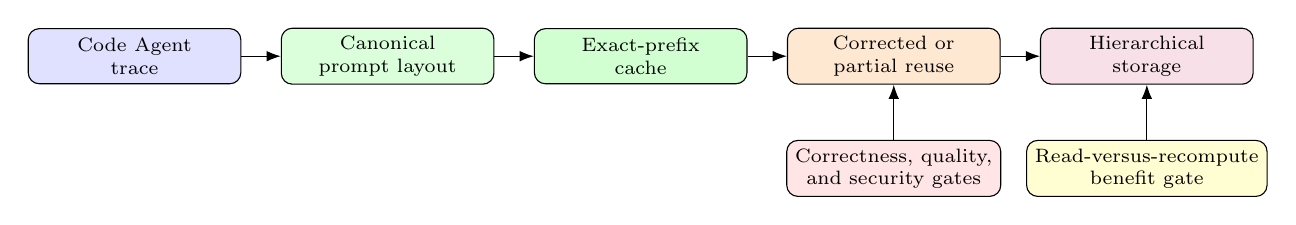
\begin{tikzpicture}[
  node distance=4mm and 5mm,
  box/.style={draw,rounded corners,minimum height=7mm,minimum width=27mm,align=center,font=\scriptsize,inner sep=3pt},
  arr/.style={-{Latex[length=1.8mm]},thin}
]
\node[box,fill=blue!12] (trace) {Code Agent\\trace};
\node[box,fill=green!14,right=of trace] (canonical) {Canonical\\prompt layout};
\node[box,fill=green!18,right=of canonical] (exact) {Exact-prefix\\cache};
\node[box,fill=orange!18,right=of exact] (partial) {Corrected or\\partial reuse};
\node[box,fill=purple!12,right=of partial] (hier) {Hierarchical\\storage};
\node[box,fill=red!10,below=7mm of partial] (quality) {Correctness, quality,\\and security gates};
\node[box,fill=yellow!18,below=7mm of hier] (benefit) {Read-versus-recompute\\benefit gate};
\draw[arr] (trace) -- (canonical);
\draw[arr] (canonical) -- (exact);
\draw[arr] (exact) -- (partial);
\draw[arr] (partial) -- (hier);
\draw[arr] (quality) -- (partial);
\draw[arr] (benefit) -- (hier);
\end{tikzpicture}
\caption{The survey taxonomy separates workload shaping, semantic reuse, and physical placement. Later mechanisms do not remove earlier correctness gates.}
\label{fig:taxonomy}
\end{figure*}

\section{Reuse Mechanisms}

\subsection{Exact-Prefix Caching}

Exact-prefix systems differ in indexing granularity, scheduling, and physical sharing. PagedAttention supplies page-granular KV memory management; vLLM automatic prefix caching hashes blocks and prefix dependencies \cite{kwon2023efficient,d01vllmproject}. SGLang's RadixAttention unifies prefix matching, sharing, and eviction within a radix tree \cite{zheng2023sglang}. TensorRT-LLM exposes reuse, offload, and priority-based retention controls \cite{d07nvidia}. Exact matching is the strongest first baseline because it admits a clear no-cache comparison and a strict correctness oracle.

\subsection{Active Prefix Construction}

Cache effectiveness is partly a context-builder property. Stable system instructions, tool definitions, and repository rules should appear before volatile content. Serialization, whitespace, file ordering, tool-schema order, and timestamps must be deterministic. Repository content should carry commit or content identifiers. Dynamic tool output and current instructions should be appended where possible. Commercial APIs similarly describe prefix-based reuse and recommend stable common content first \cite{d09openai,d10anthropic,d12google,d13deepseek}.

This strategy does not change model semantics if it preserves the intended prompt and ordering constraints. It can nevertheless change agent behavior if information is reordered, so prompt canonicalization requires task-success regression tests rather than token overlap alone.

\subsection{Position-Independent and Partial Reuse}

Non-prefix approaches seek reuse when content appears after different prefixes or at shifted positions. Their design space includes precompiling independent modules, correcting positional encodings, recomputing boundary tokens, selecting high-deviation tokens, or using an architecture whose stored representation cleanly separates position \cite{gim2023prompt,hu2024epic,ma2026irminsul}. The attraction for Code Agents is clear: file order, retrieval rank, compaction, and local edits can invalidate a long exact prefix even when most content repeats. The risk is equally clear: approximation error can alter a tool choice or patch despite small average logit error.

\subsection{Compute, Load, or Combine}

The decision need not be binary. Cake overlaps KV loading with local recomputation and adapts to the faster path \cite{jin2024compute}. This is relevant when SSD or remote bandwidth is variable. A general reuse decision is

\begin{align}
T_{load} &= T_{lookup} + \frac{B_{KV}}{BW_{eff}} + T_{restore}, \\
\text{reuse iff}\quad T_{load} + T_{risk} &< T_{recompute},
\label{eq:benefit}
\end{align}

where $T_{risk}$ is zero for an exact compatible hit but may include correction, validation, or an explicit quality penalty for approximate reuse. Equation~\ref{eq:benefit} must be evaluated per tier, size, queue state, and hardware path.

\begin{table*}[t]
\caption{Taxonomy of reuse mechanisms for Code Agent contexts.}
\label{tab:reuse}
\centering
\small
\begin{tabularx}{\textwidth}{p{0.15\textwidth}p{0.22\textwidth}p{0.20\textwidth}p{0.19\textwidth}Y}
\toprule
Mechanism & Match condition & Representative work & Main benefit & Principal risk \\
\midrule
Exact prefix & Same token prefix and execution identity & vLLM APC, SGLang, ChunkAttention & Deterministic skip of prefill for matched blocks & Fragile to early changes; block tail recomputed. \\
Structured modules & Declared reusable prompt components & Prompt Cache & Application-controlled modularity & Schema and position constraints; integration burden. \\
Canonicalized layout & Stable content rendered first and deterministically & Provider guidance; Code Agent context builders & Converts latent repetition into prefix repetition & Reordering can change behavior; requires version discipline. \\
Corrected non-prefix & Content match plus positional/boundary correction & CacheBlend, EPIC, MEPIC, KVBoost & Reuses shifted or reordered files and retrieved chunks & Approximation, correction cost, model-specific assumptions. \\
Architecture-native reuse & Representation exposes position-free reusable state & Irminsul for MLA & Lower correction width for compatible MLA implementations & Does not generalize automatically to GQA, hybrid, or opaque runtimes. \\
Compute-load overlap & Use compute and I/O concurrently & Cake & Robust to variable device or queue performance & Consumes both compute and I/O; scheduling complexity. \\
\bottomrule
\end{tabularx}
\end{table*}

\section{Hierarchical and Disaggregated KV Systems}

\subsection{Storage Tiers}

GPU memory has the lowest access latency but the smallest and most expensive capacity. Host DRAM expands capacity over PCIe or NVLink. NVMe provides much larger capacity with higher latency and sensitivity to request size and layout. Remote memory or storage enables sharing across nodes but adds network and coordination costs. The appropriate object to place is usually a block or chunk with metadata, not an untyped tensor dump.

\begin{figure}[t]
\centering
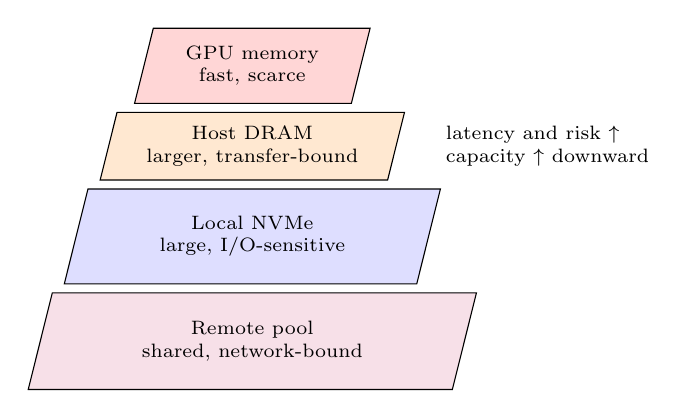
\begin{tikzpicture}[
  tier/.style={trapezium,trapezium left angle=76,trapezium right angle=104,draw,align=center,font=\scriptsize,minimum height=7mm},
  note/.style={font=\scriptsize,align=left}
]
\node[tier,fill=red!16,minimum width=30mm] (gpu) {GPU memory\\fast, scarce};
\node[tier,fill=orange!18,minimum width=39mm,below=1mm of gpu] (dram) {Host DRAM\\larger, transfer-bound};
\node[tier,fill=blue!13,minimum width=48mm,below=1mm of dram] (ssd) {Local NVMe\\large, I/O-sensitive};
\node[tier,fill=purple!12,minimum width=57mm,below=1mm of ssd] (remote) {Remote pool\\shared, network-bound};
\node[note,right=5mm of dram] {latency and risk $\uparrow$\\capacity $\uparrow$ downward};
\end{tikzpicture}
\caption{A logical KV hierarchy. Real ordering depends on interconnect, device, serialization, and access size.}
\label{fig:hierarchy}
\end{figure}

Mooncake treats distributed KV storage as a first-class serving substrate, trading storage for less computation \cite{qin2025mooncake}. MemServe introduces an elastic pool across CPU and GPU memory \cite{hu2024memserve}. LMCache exposes lookup, movement, offload, compression, and cross-engine sharing \cite{liu2025lmcache,d05lmcacheproject}. Strata focuses on long-context hierarchical caching and fragmented I/O, while HiCache extends RadixAttention beyond GPU memory \cite{xie2025strata,d03sglangproject}. Tutti and KVDrive further target SSD-backed and multi-tier operation \cite{qiu2026tutti,lin2026kvdrive}.

\subsection{Prefill-Decode Disaggregation}

DistServe assigns prefill and decode to different GPU pools to reduce interference and independently satisfy \ttft and \tpot objectives \cite{zhong2024distserve}. FlowKV emphasizes low-latency KV transfer and load-aware scheduling \cite{li2025flowkv}. Disaggregation increases the importance of transfer layout, network bandwidth, and routing. It should not be conflated with inter-request reuse: a KV object may be transferred once between prefill and decode without ever serving another request.

\subsection{Data Movement and Layout}

CacheGen compresses KV for bandwidth-adaptive streaming \cite{liu2023cachegen}. InfiniGen dynamically selects and stages KV from host memory, and FlexGen provides a broader single-GPU offloading baseline \cite{lee2024infinigen,sheng2023flexgen}. Paged GPU layouts may cause small, fragmented transfers; hierarchical systems therefore aggregate blocks, decouple layouts across tiers, pipeline movement with compute, or use GPU-assisted I/O.

\begin{table*}[t]
\caption{Representative systems and the layer they optimize.}
\label{tab:systems}
\centering
\scriptsize
\begin{tabularx}{\textwidth}{p{0.12\textwidth}p{0.18\textwidth}p{0.17\textwidth}p{0.21\textwidth}Y}
\toprule
System & Primary abstraction & Tiers or topology & Reuse/transfer role & Code Agent relevance \\
\midrule
vLLM / PagedAttention & Paged GPU KV blocks & GPU; connectors in current ecosystem & Memory management and exact-prefix APC & Strong no-cache/APC baseline on one node. \\
SGLang / RadixAttention & Radix tree over shared token prefixes & GPU; extended by HiCache & Exact-prefix lookup, sharing, scheduling, eviction & Natural fit for growing multi-turn histories. \\
MemServe & Elastic distributed memory pool & GPU and CPU across instances & Inter-request cache plus disaggregated transfer & Evaluates shared context across workers. \\
Mooncake & KV-centric distributed store & GPU, DRAM, SSD, NIC resources & Persistent distributed cache and scheduling & Reference for scale-out capacity and storage-compute tradeoff. \\
LMCache & Engine-independent KV layer and connectors & GPU, CPU, local/remote storage & Cross-query offload and cross-engine movement & Useful instrumentation and pluggable prototype layer. \\
Strata / HiCache & Hierarchical context cache & HBM, host DRAM, disk or external store & Cache-aware loading, prefetch, and scheduling & Directly targets long repeated contexts and deep tiers. \\
DistServe / FlowKV & Separate prefill and decode workers & GPU pools plus interconnect & Intra-request KV handoff & Relevant when scaling beyond a single RTX 5090 node. \\
CacheGen & Encoded KV stream & Storage/network to GPU & Transfer compression and adaptation & Tests whether compressed loading beats recompute. \\
Cake & Concurrent load and compute & GPU plus storage path & Adaptive bidirectional completion & Provides a practical effective-hit decision baseline. \\
\bottomrule
\end{tabularx}
\end{table*}

\section{Compression, Eviction, and Architecture}

\subsection{Four Compression Axes}

Compression methods change different objects and should not be compared by a single ``compression ratio.''

\begin{enumerate}
    \item \emph{Token retention}: H2O, Scissorhands, StreamingLLM, SnapKV, PyramidKV, and DuoAttention retain selected tokens or distinguish attention-head behaviors \cite{zhang2023heavyhitter,liu2023scissorhands,xiao2023efficient,li2024snapkv,cai2024pyramidkv,xiao2024duoattention}.
    \item \emph{Numerical precision}: KIVI, KVQuant, QAQ, SKVQ, MiniKV, and PQCache use low-bit or product quantization with different granularity and outlier handling \cite{liu2024kivi,hooper2024kvquant,dong2024quality,duanmu2024skvq,sharma2024minikv,zhang2024pqcache}.
    \item \emph{Dimension or layer reduction}: MiniCache merges similar cross-layer states and FDC compresses KV dimensions while targeting attention efficiency \cite{liu2024minicache,zhang2024fast}.
    \item \emph{Transfer encoding}: CacheGen optimizes serialized KV movement rather than only in-GPU attention \cite{liu2023cachegen}.
\end{enumerate}

These techniques can be complementary, but combinations multiply metadata, conversion, and kernel requirements. Production-oriented evaluation has warned that nominal memory savings can fail to improve throughput and may even increase end-to-end latency \cite{gao2025rethinking}.

\subsection{Architecture Changes the Cache Object}

MQA shares one set of K/V heads across query heads; GQA generalizes this to groups \cite{shazeer2019fast,ainslie2023training}. MLA compresses token state into latent representations and changes how positional components are handled \cite{deepseekai2024deepseekv,deepseekai2024deepseekv2}. DeepSeek-V3.2 introduces dynamic sparse attention in a model family that already uses MLA \cite{deepseekai2025deepseekv}. Hybrid attention or state-space models may alternate full attention, local attention, sparse attention, and recurrent state. A unified cache API is possible, but a single opaque tensor format is not.

At minimum, serialized metadata should include model and weight revision, layer and attention type, tensor shape and strides, token range, KV-head or latent layout, position encoding, dtype, quantization scales and grouping, sparsity indexes, adapter identity, checksum, and security domain. Compatibility should be declared per model revision and kernel path.

\begin{table*}[t]
\caption{Compression and architecture interactions.}
\label{tab:compression}
\centering
\small
\begin{tabularx}{\textwidth}{p{0.15\textwidth}p{0.20\textwidth}p{0.20\textwidth}p{0.19\textwidth}Y}
\toprule
Class & Reduced dimension & Example methods & Required quality check & Reuse interaction \\
\midrule
Token eviction & Sequence positions & H2O, Scissorhands, SnapKV, PyramidKV & Long-context retrieval, code-task success, output length & A cached object is approximate and may be query-dependent. \\
Low-bit quantization & Bits per K/V element & KIVI, KVQuant, QAQ, SKVQ, MiniKV & Logit error, generation agreement, task success & Expands capacity and reduces transfer bytes; adds conversion and scale metadata. \\
Cross-layer/dimension & Layers or vector width & MiniCache, FDC & Per-model quality and kernel throughput & Format can be incompatible with standard cache connectors. \\
Transfer encoding & Bytes on storage/network path & CacheGen & End-to-end load latency and reconstruction quality & Useful for lower tiers even if GPU attention remains high precision. \\
Architectural sharing & Number or form of KV heads/state & MQA, GQA, MLA, DSA/hybrid & Model-native accuracy and runtime compatibility & Changes size formula, position correction, serialization, and potential sharing semantics. \\
\bottomrule
\end{tabularx}
\end{table*}

\section{Admission, Placement, and Eviction}

Saving every generated block can waste storage and I/O. A reusable admission score should incorporate reuse probability, recomputation cost, object size, load cost, and quality/security risk. One useful abstraction is

\begin{equation}
V_i = \frac{p_i^{reuse}\,C_i^{recompute}-C_i^{load}-C_i^{risk}}
{B_i\,\tau_i},
\label{eq:value}
\end{equation}

where $B_i$ is stored bytes and $\tau_i$ a retention or tier-cost factor. The exact estimator is a research question; Equation~\ref{eq:value} prevents a raw hit count from dominating all other objectives.

Placement can be formulated as a constrained decision over GPU, host, SSD, remote, or drop. Hot adjacent-turn prefixes belong near the GPU. Repository content with slower reuse may fit DRAM or SSD. Platform-shared system prompts can be pinned only if the security domain permits sharing. Prefetch should use session, repository, agent step, and queue signals, while preserving a fallback to recomputation.

LRU is an essential baseline but ignores object size and saved compute. Priority-aware retention in current TensorRT-LLM and cache-aware scheduling in SGLang or hierarchical systems provide practical comparison points \cite{d07nvidia,d03sglangproject}. Any learned policy must be compared with LRU, size-aware LRU, GreedyDual-style value policies, and an oracle derived from replay.

\section{Evaluation Methodology}

\subsection{Hit Metrics}

Request hit rate alone is weak because a one-block reuse and a nearly complete prefill both count as hits. At least three levels are required:

\begin{align}
H_{req} &= \frac{N(\text{requests with any reuse})}{N(\text{requests})}, \\
H_{tok} &= \frac{N(\text{reused prefill tokens})}{N(\text{prompt tokens})}, \\
H_{eff} &= \frac{N(\text{profitably reused tokens})}{N(\text{prompt tokens})}.
\label{eq:hits}
\end{align}

A token is profitable only if it passes Equation~\ref{eq:benefit}. Results should be decomposed by tier, exact versus approximate reuse, tenant scope, context length, and cold/warm state. LMCache exposes request- and token-oriented observability concepts that can inform instrumentation \cite{d06lmcacheproject}.

\subsection{Latency, Throughput, Cost, and Quality}

The main latency gain is

\begin{equation}
G_{TTFT}=\frac{TTFT_{base}-TTFT_{cache}}{TTFT_{base}}.
\label{eq:ttft}
\end{equation}

Report P50, P95, and P99 \ttft, prefill time, queue time, lookup, bytes transferred, restoration, and correction. Decode \tpot must remain visible because prefill scheduling can interfere with decode. Throughput should include requests/s, input tokens/s, output tokens/s, and goodput under explicit SLOs.

End-to-end cost should include GPU time, CPU and DRAM, storage, network, and cache-management overhead:

\begin{equation}
C_{ratio}=\frac{C_{GPU}+C_{CPU}+C_{store}+C_{net}+C_{ops}}
{C_{baseline}}.
\label{eq:cost}
\end{equation}

Exact reuse should be checked against a no-cache oracle for logits or generated tokens under controlled determinism. Approximate reuse additionally requires repository-task success, test outcomes, long-context benchmarks, and sensitivity to output length. LongBench and RULER are useful generic controls but cannot replace Code Agent task success \cite{bai2023longbench,hsieh2024ruler}.

\begin{table}[t]
\caption{Minimum evaluation dimensions.}
\label{tab:metrics}
\centering
\small
\begin{tabularx}{\columnwidth}{p{0.26\columnwidth}Y}
\toprule
Dimension & Required reporting \\
\midrule
Correctness & Exact-cache consistency; logit or token agreement; test and task success. \\
Reuse & Request, token, effective hit rates; prefix/non-prefix; tier; tenant scope. \\
Latency & Prefill, \ttft P50/P95/P99, lookup, transfer, restore, correction, \tpot. \\
Capacity & Bytes/token, resident bytes by tier, metadata, fragmentation, compression ratio. \\
Throughput & Requests/s, input/output tokens/s, goodput under \ttft and \tpot SLOs. \\
Cost & GPU, CPU, DRAM, storage, network, operations, and per-million-token cost. \\
Security & Isolation policy, cache-key domain, probe leakage, retention, deletion. \\
\bottomrule
\end{tabularx}
\end{table}

\subsection{Replay Design}

A credible experiment needs both real or near-real trajectories and controlled synthetic traces. Real traces establish external validity; synthetic traces isolate mechanisms. Controlled axes should include context length, exact-prefix fraction, shifted repetition, edit location, file order, cache capacity, tier, concurrency, inter-arrival time, and repository version.

The minimum record should contain run and request IDs, timestamp, session, tenant and repository IDs, commit, task class, rendered prompt, token IDs or a privacy-preserving equivalent, segment type and order, model/tokenizer/adapter identity, cache lookup and transfer events, tier, bytes, timing, output, tool action, test result, and file changes. Sensitive source and logs require access control and configurable retention.

\subsection{Hardware Interpretation}

The project's current first-node assumption is Ubuntu with one GeForce RTX 5090, 32 GB GDDR7, and 64 GB system memory; a larger HBM-based server remains tentative. The official GPU specification should be recorded rather than describing the 5090's device memory as HBM \cite{d18nvidia}. This node can support a single-GPU baseline and GPU-to-host experiments, with local NVMe added if specified. It cannot validate multi-node RDMA, shared remote cache, or HBM-cluster claims. Those require a separate environment and should not be inferred from single-node results.

\section{Security, Privacy, and Isolation}

Cross-user cache sharing creates state-dependent timing. Auditing work shows that cache-hit timing can reveal whether a prefix has been cached \cite{gu2025auditing}. SafeKV and CachePrune explore selective sharing or fine-grained privacy-aware reuse \cite{chu2025selective,wu2026cacheprune}. Other work studies direct KV reconstruction, prefix-cache isolation, gateway auditing, and new attack surfaces in position-independent reuse \cite{luo2025shadow,pennas2026prefixwall,fahey2026cacheprobe,zhang2026hijackkv}.

The safest initial policy is isolation by default: a cache key includes tenant or principal identity, and cross-tenant sharing is limited to explicitly public, immutable content such as platform-controlled instructions. Hash salting, access-control checks, encryption at rest and in transit, deletion semantics, audit logs, and timing analysis are system requirements, not optional add-ons. A high hit rate does not justify crossing an undefined security boundary.

\section{Research Gaps for Code Agents}

\subsection{Public Trace Gap}

Agent benchmarks expose tasks and success, but few publish the exact sequence of fully rendered prompts, tokenized segments, cache events, and hardware timing needed for replay. A privacy-conscious Code Agent cache trace format is therefore a useful research artifact in its own right.

\subsection{Context-Builder and Cache Co-Design}

Existing serving research usually treats prompts as given. Code Agents actively assemble context from repository search, memory, tool schemas, and compaction. The open question is how to maximize stable prefixes without degrading task quality or starving the model of relevant context. Context retrieval benchmarks and repository methods provide inputs to this co-design but do not optimize KV reuse directly \cite{li2026contextbench,liu2023repobench,zhang2023repocoder}.

\subsection{Dependency-Aware Invalidation}

When one file changes, exact-prefix systems invalidate all later blocks even if most repository content is unchanged. Arbitrary preservation is unsafe because causal state carries earlier dependencies. Research is needed on dependency-aware layout, explicit module boundaries, positional correction, selective recomputation, and validation that measures tool decisions and code-task success rather than only language-model similarity.

\subsection{Architecture-Portable Cache Objects}

GQA, MLA, DSA, multimodal, and hybrid models do not share one physical cache representation. A portable object model should make incompatibility explicit and support conversion only when correctness, metadata, and kernels are defined. The project term ``TensorQuant'' does not identify a single public KV format and must remain an unresolved requirement until a specification is provided.

\subsection{Benefit-Aware Hierarchy}

The boundary between recomputation and load changes with prompt length, GPU generation, PCIe or NVLink, SSD access size, network congestion, compression, queue depth, and concurrent decode. Static tier thresholds are unlikely to generalize. Online benefit models should be calibrated, compared with Cake-like overlap, and evaluated on tail latency, not just averages.

\subsection{Security-Preserving Reuse}

Position-independent and fine-grained sharing increase the number of matchable fragments and potentially the observable cache surface. Security domains, salted indexing, visibility labels, and constant- or noise-shaped response policies must be evaluated together with hit rate.

\section{Implications for the Proposed Project}

The evidence supports a research sequence, not an immediate full implementation:

\begin{enumerate}
    \item \textbf{Trace and measurement first.} Define Code Agent task classes, collect replayable trajectories, and quantify exact prefix, shifted repetition, edit locality, and context churn.
    \item \textbf{Exact baseline second.} Compare no-cache and engine-native exact-prefix caching with identical model, scheduler, and workload settings. Establish correctness and latency decomposition.
    \item \textbf{Context-layout study third.} Test deterministic rendering, stable-first ordering, repository versioning, and controlled compaction. Measure both task success and reusable-token gain.
    \item \textbf{Hierarchy study fourth.} Add host DRAM and then NVMe only after transfer-versus-recompute models are calibrated. Multi-node or HBM-server claims wait for the corresponding hardware.
    \item \textbf{Research mechanisms last.} Study dependency-aware invalidation, position-independent reuse, quantized transport/storage, and architecture portability with explicit quality and security gates.
\end{enumerate}

Table~\ref{tab:agenda} maps claims to evidence required. This prevents a logical hit rate from being substituted for end-to-end benefit.

\begin{table*}[t]
\caption{Claim-to-evidence matrix for the project.}
\label{tab:agenda}
\centering
\small
\begin{tabularx}{\textwidth}{p{0.20\textwidth}p{0.25\textwidth}p{0.24\textwidth}Y}
\toprule
Proposed claim & Required denominator and baseline & Minimum evidence & Invalid shortcut \\
\midrule
High Code Agent cache hit rate & All prefill tokens in declared task distribution & Real trace, model/tokenizer identity, tiered $H_{tok}$ and $H_{eff}$ & Request hit rate or text repetition alone. \\
At least 90\% \ttft reduction on hits & Matched no-cache requests under same concurrency & P50/P95/P99 and lookup/transfer/restore breakdown & Comparing warm cache to cold model startup. \\
Inference cost below 10\% & End-to-end cost with cache infrastructure & GPU, CPU, memory, storage, network, and operation accounting & GPU prefill FLOPs alone. \\
Safe partial reuse & Full recomputation oracle & Logit/token checks plus repository-task and test success & Text similarity or average perplexity only. \\
Architecture compatibility & Each named model revision and runtime path & Tensor schema, metadata, kernel, quantization, position, and quality tests & Treating every architecture as a standard K/V tensor. \\
Multi-tenant sharing & Explicit trust and visibility policy & Isolation tests, timing audit, retention/deletion, access logs & Hashing private content without a tenant domain. \\
\bottomrule
\end{tabularx}
\end{table*}

The proposed numerical targets - general hit rate of 70\%, Code Agent hit rate of 95\%, hit-path \ttft reduction of 90\%, and cost ratio no greater than 10\% - are not established by the surveyed literature for the target workload. They should remain acceptance hypotheses until the measurement protocol, denominator, trace, and hardware are fixed.

\section{Conclusion}

Code Agents are unusually attractive for KV reuse because they make repeated, dependent model calls over stable instructions, tool schemas, histories, and mostly unchanged repositories. The most defensible first mechanism is exact-prefix caching under a complete execution-identity key, strengthened by deterministic context construction. The research frontier begins where exact prefixes break: reordered files, local edits, compaction, heterogeneous cache formats, deep storage tiers, and multi-tenant sharing.

The literature shows that no single hit rate captures this system. Correctness, token coverage, tier location, transfer cost, tail latency, task quality, and isolation must be measured together. Hierarchical storage and compression expand capacity only when their I/O and conversion paths beat recomputation. Non-prefix reuse expands opportunity only when positional and causal dependencies are repaired or proven irrelevant. For the proposed project, the immediate outcome of this survey is therefore a trace-driven research agenda and a disciplined baseline hierarchy, not a claim that ambitious targets have already been met.

\section*{Corpus Note}

The accompanying research package indexes all 76 papers reviewed here, including additional repository benchmarks, multimodal caching, compression variants, and recent security studies \cite{yang2024swebench,zhang2025swebench,zan2025multiswebench,pan2024training,liang2024repofuse,liu2024graphcoder,zhao2025mpic,chen2026packet,wang2025mepic,zhang2026sparsex,sharma2024minikv,duanmu2024skvq,zhang2024pqcache}. It also preserves 18 official documentation links and machine-readable metadata, abstracts, BibTeX, licenses, and checksums.

\begingroup
\sloppy
\emergencystretch=2em
\hfuzz=1pt
\bibliographystyle{ieeetr}
\bibliography{references}
\endgroup

\end{document}
